\begin{correction}   \;
\begin{enumerate}
\item La fonction $f$ est bien d\'efinie si et seulement si $2x\not= 0$ et ainsi $\mathcal{D}_f=\R^{\star}$. La fonction $f$ est d\'erivable sur $\R^{\star}$ comme somme et quotient dont le d\'enominateur ne s'annule pas de fonctions d\'erivables. De plus, pour tout $x\not= 0$, on a: $f^{\prime}(x)=\ddp\frac{-1}{2x^2}$. 
\item 
\begin{itemize}
\item[$\bullet$] Limites en $\pm\infty$: $\lim\limits_{x\to +\infty}  f(x)=-\ddp\demi=\lim\limits_{x\to -\infty}  f(x)$ d'apr\`{e}s le th\'eor\`{e}me des monomes de plus haut degr\'e. La courbe $\mathcal{C}_f$ admet une asymptote horizontale d'\'equation $y=-\ddp\demi$ au voisinage de $\pm\infty$.
\item[$\bullet$] Limites en $0$: $\lim\limits_{x\to 0^+} f(x)=+\infty$ et $\lim\limits_{x\to 0^-} f(x)=-\infty$ par propri\'et\'es sur les somme et quotient de limites. La courbe $\mathcal{C}_f$ admet une asymptote verticale d'\'equation $x=0$. 
\end{itemize}
On obtient alors le tableau de variation suivant:
\begin{center}
 \begin{tikzpicture}
 \tkzTabInit{ $x$          /1,%
      $f^{\prime}(x)$   /1,
       $f$       /2}%
     { $-\infty$,$0$,$+\infty$}%
   \tkzTabLine{ ,-,d,-,}
  \tkzTabVar{
       +/$-\demi$            /,
        -D+/ $-\infty$ /$+\infty$    /,
        -/ $-\demi$          /
                      }                 
\end{tikzpicture}
\end{center}
\item D\'ej\`{a} fait \`{a} la question pr\'ec\'edente.
\item La fonction $f$ est d\'erivable en 1 ainsi la tangente $T_1$ \`{a} la courbe au point d'abscisse 1 existe bien et son \'equation est: $y=f^{\prime}(1)(x-1)+f(1)$. Les calculs donnent: $y=-\ddp\demi(x-1)$. 
\item 
\begin{itemize}
\item[$\bullet$] Le domaine de d\'efinition est bien centr\'e en 0 car: $\forall x\in\R^{\star}, -x\in\R^{\star}$.
\item[$\bullet$] Soit $x\in\R^{\star}$, on a: $f(-x)=\ddp\frac{x+1}{-2x}=-\ddp\frac{x+1}{2x}$ et 
$-1-f(x)=\ddp\frac{  -2x+x-1 }{2x}=-\ddp\frac{x+1}{2x}$. Ainsi, on a bien: $f(-x)=-1-f(x)$. 
\end{itemize}
On cherche alors une sym\'etrie $s$ entre les points $(x,f(x))$ et $(-x, f(-x))$ sur le graphe de $f$, soit $s$ telle que $(-x,f(-x)) = s(x,f(x))$. Pour cela, essayons de trouver quelles conditions doit v\'erifier $(x,f(x))$ pour que le point soit inchang\'e par la sym\'etrie. Le point $(x,f(x))$ est un point fixe de $s$ si on a $s(x,f(x)) = (x,f(x))$. Or $s(x,f(x))=(-x,f(-x))$, donc on doit avoir :
$$\left\{ \begin{array}{rcl}
-x &=& x\vsec\\
f(-x) & = & f(x)
\end{array}\right. \; \Leftrightarrow
\;\left\{ \begin{array}{rcl}
2x &=& 0\vsec\\
-1-f(x) & = & f(x)
\end{array}\right. \; \Leftrightarrow
\;\left\{ \begin{array}{rcl}
x &=& 0\vsec\\
f(x) & = & \ddp -\frac{1}{2}
\end{array}\right. $$ 
Le seul point fixe de la transformation est $\Omega\left( 0,-\ddp\demi \right)$. On v\'erifie alors que l'on a bien : $\ddp \frac{x+(-x)}{2}=0$ et $\ddp \frac{f(x)+f(-x)}{2} = - \frac{1}{2}$, autrement dit que $\Omega$ est le milieu entre les points $(x,f(x))$ et $(-x, f(-x))$. On obtient alors que la courbe $\mathcal{C}_f$ est sym\'etrique par rapport au point $\Omega\left( 0,-\ddp\demi \right)$.
\item Graphe de $f$ :
%\begin{center}
%\includegraphics[width=0.5\linewidth]{./ex16.eps} 
%\end{center}
\item On a pour tout $x\in\R^{\star}$: $f(x)=x\Leftrightarrow f(x)-x=0 \Leftrightarrow \ddp\frac{-x+1-2x^2}{2x}=0\Leftrightarrow -2x^2-x+1=0$. Le discriminant vaut $\Delta=9$ et les deux racines sont $-1$ et $\ddp\demi$. Ces solutions correspondent aux abscisses des points fixes pour la fonction $f$.
\end{enumerate}
\end{correction}

%--------------------------------------------------
%------------------------------------------------
